\documentclass[tikz,border=10pt]{standalone}
\usepackage{tikz}
\usetikzlibrary{positioning}
\usepackage{tikz-feynman}
\usetikzlibrary{graphs}
\begin{document}

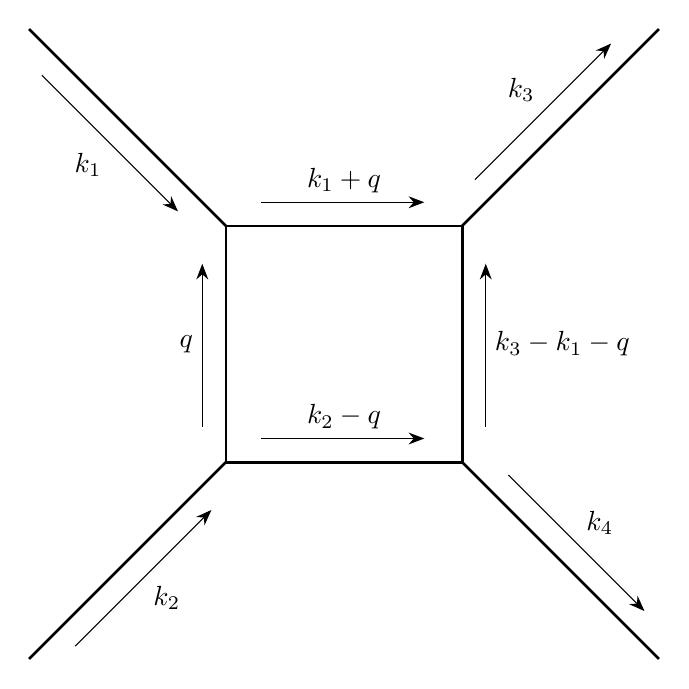
\begin{tikzpicture}
	\begin{feynman}
		\vertex (a1);
		\vertex[above =3cm  of a1] (a2);
		\vertex[left =3cm  of a2] (a3);
		\vertex[below =3cm  of a3] (a4);
		\vertex[below right =2.5cm and 2.5cm  of a1] (a5);
		\vertex[above right =2.5cm and 2.5cm  of a2] (a6);
		\vertex[above left =2.5cm and 2.5cm  of a3] (a7);
		\vertex[below left =2.5cm and 2.5cm  of a4] (a8);
		\diagram*{
		{ [edge={line width=1pt}]
		(a4) --[momentum={[arrow style=black]\(q\)}]
		(a3) --	[momentum={[arrow style=black]\(k_{1}+q\)}]
		(a2),
		(a4) --[momentum={[arrow style=black]\(k_{2}-q\)}]
		(a1) --[momentum'={[arrow style=black]\(k_{3}-k_{1}-q\)}]
        (a2),
        %%%%%%%%%%
		(a3)--[reversed momentum={[arrow style=black]\(k_{1}\)}]
        (a7),
        (a4)--[reversed momentum={[arrow style=black]\(k_{2}\)}]
        (a8),
        %%%%%%%%%%
		(a2)--[ momentum={[arrow style=black]\(k_{3}\)}]
		(a6),
		(a1)--[ momentum={[arrow style=black]\(k_{4}\)}]
		(a5),
		},
		};
	\end{feynman}
\end{tikzpicture}
\end{document}
